%-----------------------------------------------------------------------------%
\chapter{\babSatu}
%-----------------------------------------------------------------------------%
Pada bagian ini akan dijelaskan latar belakang dari pengerjaan tugas akhir ini, tujuan penulisan, rumusan masalah, ruang lingkup dan batasan pengerjaan, tahapan pengerjaan, dan sistematika penulisan laporan.


%-----------------------------------------------------------------------------%
\section{Latar Belakang}
%-----------------------------------------------------------------------------%
Penemuan internet beberapa dekade lalu telah merubah cara manusia dalam hal bertukar informasi. Popularitas dari internet terus meningkat hingga pada akhirnya, menurut data dari cisco\cite{CiscoIot}, jumlah perangkat yang terhubung ke internet pada tahun 2010 telah melewati jumlah dari populasi manusia yang ada di Bumi. Lebih jauh lagi, diperkirakan pada tahun 2015 ini jumlah perangkat yang terhubung ke internet akan menjadi dua kali lipat dari jumlah populasi manusia. Hal ini disebabkan oleh teknologi komputer terbenam (komputer yang tidak terlihat keberadaannya) yang akan memicu lahirnya era baru dalam sejarah internet, era \iot.

Saat ini, berbagai perangkat yang menerapkan konsep \iot~telah bermunculan di pasaran. Beberapa \textit{platform} yang bertujuan menghubungkan berbagai perangkat \iot-pun mulai bermunculan di pasaran. Berbagai \textit{platform} tersebut memiliki berbagai pendekatan, mulai dari yang menargetkan \textit{end-user} dengan model otomasi, sampai yang menargetkan konsumen \textit{enterprise}. Salah satu pendekatan yang belum banyak terlihat keberadaanya di pasaran adalah pendekatan dengan model sosial media dan menargetkan pada \textit{end-user}. Oleh karena itu, \saya~dan teman-teman \saya~tertarik untuk mengembangkan sebuah \plat~\iot~yang menggunakan model sosial media dan ditargetkan untuk \textit{end-user}.

Untuk membuat sebuah \textit{platform} yang menargetkan pada \textit{end-user}, diperlukan cara untuk menghubungkan berbagai perangkat yang dimiliki konsumen dengan cara yang mudah. Mekanisme pendaftaran ini harus bisa menangani baik perangkat yang sudah beredar dipasaran maupun yang nantinya akan beredar di pasaran. Konsumen juga mungkin akan menginginkan agar perangkat yang mereka miliki walaupun berbeda merek, namun bisa dikendalikan secara bersamaan. Untuk itu, dibutuhkan sebuah \textit{gateway} yang dapat menghubungkan berbagai perangkat berbeda ke \textit{platform} yang diinginkan melalui internet.

Nisrina Luthfiyati dalam tugas akhirnya yang berjudul "Implementasi ZigBee \textit{Coordinator} dengan REST \textit{Interface}"\cite{SkripsiNina} telah berhasil membuat sebuah \textit{coordinator} untuk perangkat berbasis ZigBee yang dapat diakses melalui perintah REST. Fauziah Rahmawati kemudian dalam tugas akhirnya yang berjudul "Implementasi \textit{Home Automation Gateway} untuk IOT \textit{Cloud Service} berbasis ZigBee \textit{Network}"\cite{SkripsiFarah} berhasil melanjutkan tugas akhir Nisrina Luthfiyati dan membuat sebuah \textit{gateway} yang dapat menghubungkan perangkat berbasis \textit{ZigBee} dengan \textit{Home Automation Profile} ke internet. \textit{Gateway} yang digunakan oleh Fauziah Rahmawati menerapkan konsep \textit{publish-subscribe} dalam melakukan pengiriman data ke internet.

Namun, penulis merasa masih ada yang bisa ditingkatkan dari implementasi \textit{gateway} yang telah dibuat oleh Fauziah, terutama jika akan digunakan pada \textit{platform} \iot~yang akan dibuat oleh \saya~dan teman-teman \saya~yang menargetkan pada \eu. Implementasi \textit{gateway} yang telah dibuat oleh Fauziah masih cukup rumit untuk digunakan dan masih membutuhkan suatu komputer terpisah yang terus menyala untuk bisa digunakan. Sedangkan jika ingin bisa digunakan oleh \eu, \textit{gateway} harus bisa mendaftarkan perangkat yang dimiliki konsumen dengan cara yang mudah dan bisa terhubung dengan pengelola perangkat yang ada pada \plat~terkait. \textit{Gateway} harus menyertakan identitas ketika terhubung ke \plat~sehingga dapat dibedakan antar \textit{gateway} yang dimiliki oleh \textit{user} berbeda. \textit{Gateway} juga harus memiliki bentuk yang ringkas dan tidak memerlukan komputer tambahan sehingga tidak perlu ada komputer konsumen yang menyala terus-menerus. Oleh karena itu, \saya~terpikir untuk membuat sebuah implementasi ZigBee \textit{gateway} berbasis GUI (\textit{Graphical User Interface}) dengan menggunakan Raspberry Pi untuk menyelesaikan masalah yang disebutkan sebelumnya.


%-----------------------------------------------------------------------------%
\section{Rumusan Masalah}
%-----------------------------------------------------------------------------%
Masalah yang ingin diselesaikan dalam tugas akhir ini adalah bagaimana membuat sebuah \textit{gateway} yang dapat menghubungkan perangkat yang dimiliki konsumen dengan \plat~\iot~yang menggunakan pendekatan sosial media. \textit{Gateway} harus bisa digunakan oleh \eu~dengan mudah dan dapat berkomunikasi dengan \plat~yang diinginkan. Secara spesifik, rumusan masalah dalam tugas akhir ini dapat dituangkan ke dalam pertanyaan-pertanyaan berikut:
\begin{enumerate}
	\item Bagaimana membuat ZigBee \textit{gateway} berbasis GUI dengan menggunakan Raspberry Pi?
	\item Bagaimana model komunikasi yang baik agar \textit{gateway} dapat terhubung dengan \plat~\iot~berbasis sosial media?
\end{enumerate}

%-----------------------------------------------------------------------------%
\section{Tujuan}
%-----------------------------------------------------------------------------%
Tujuan dari tugas akhir ini adalah menghasilkan sebuah perangkat \textit{gateway} yang dapat mengirimkan informasi dari jaringan lampu ZigBee ke internet. Perangkat \textit{gateway} yang dihasilkan dapat dioperasikan menggunakan GUI. \textit{Gateway} juga dikembangkan dengan berpatokan pada \plat~\iot~yang berbasis sosial media. 

\section{Posisi Penelitian}

Tugas akhir ini merupakan salah satu bagian dari satu topik besar, yaitu \textit{Social Internet of Things platform} dengan pendekatan menggunakan \textit{social media}. Pengerjaan topik besar ini dilakukan dalam satu kelompok yang dibimbing oleh Bapak Bob Hardian, seorang dosen di Fakultas Ilmu Komputer UI. Arsitektur \plat~yang akan dibuat bisa dilihat pada gambar \ref{fig:arsitektur-siot}.

\begin{figure}
	\centering
	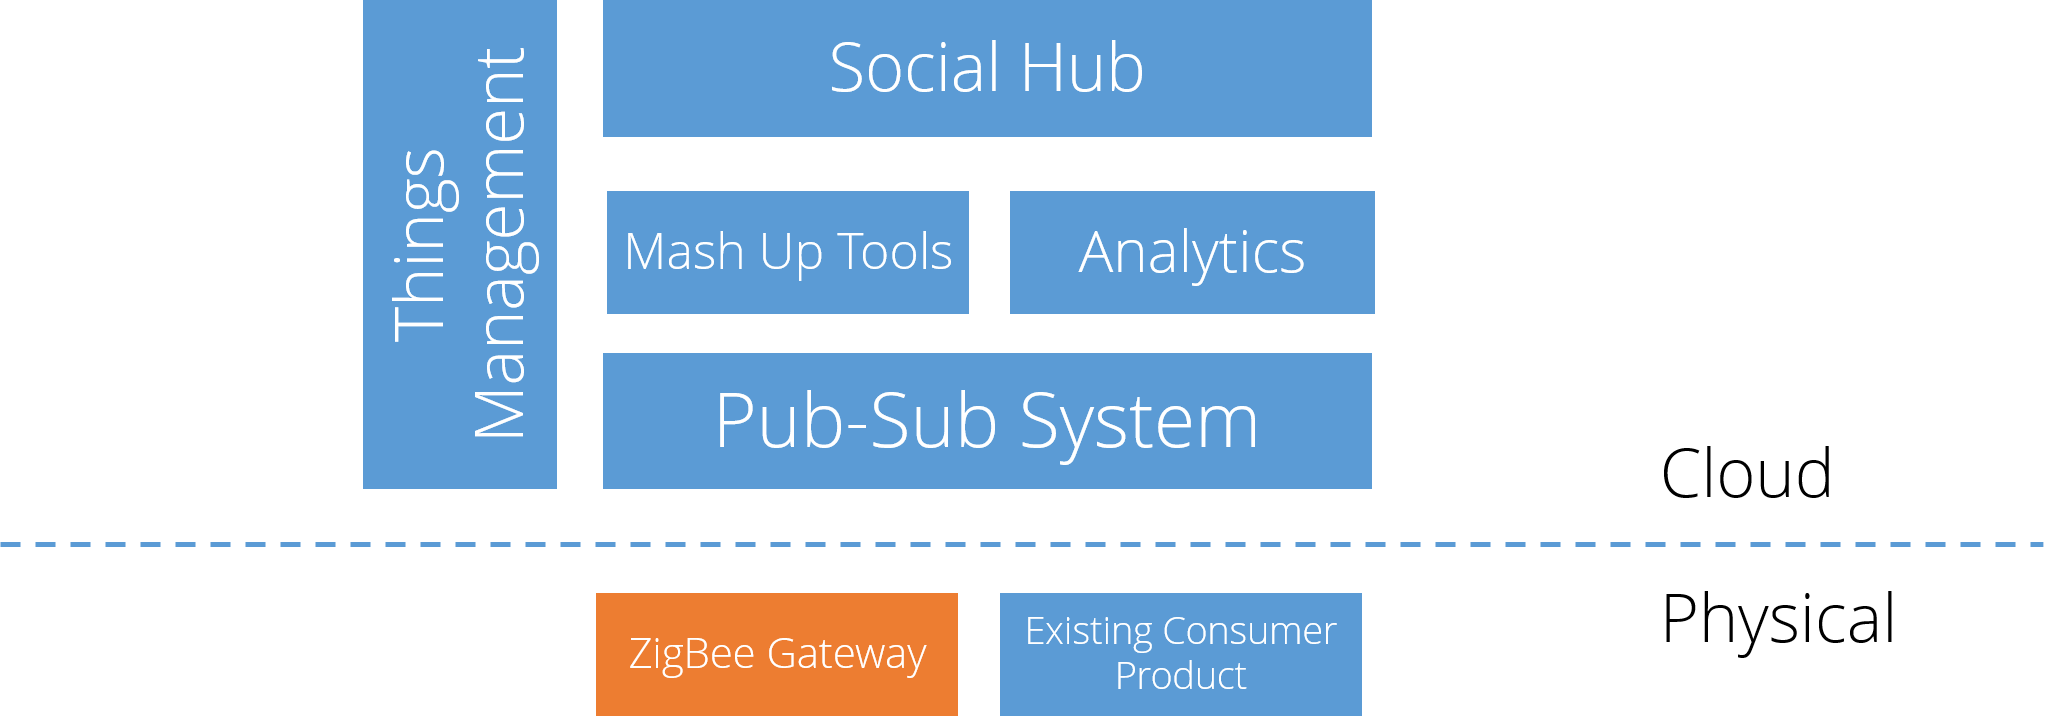
\includegraphics[width=.9\textwidth]{pics/rancangan-siot.PNG}
	\caption{Arsitektur \textit{platform} yang dibuat}
	\label{fig:arsitektur-siot}
\end{figure}

Penjelasan lebih mendetail akan dijelaskan pada Bab 3. Pembagian topik lebih spesifik dari topik besar tersebut adalah:
\begin{enumerate}
	\item \textit{Social Hub} akan dikerjakan oleh Jouvy Alif Pradewo.
	\item \textit{Mash Up Tools} akan dikerjakan oleh Muhammad Redho Ayassa.
	\item \textit{Analytics} Bagian ini belum akan dikerjakan.
	\item \textit{Pub-Sub System} akan dikerjakan oleh Abdullah Izzuddiin Alqassam.
	\item \textit{Things Management} akan dikerjakan oleh Prakoso Adi Nugroho.
	\item \textit{ZigBee Gateway} akan oleh dikerjakan oleh \saya~, Luqman Sungkar dalam tugas akhir ini.
	
\end{enumerate}

%-----------------------------------------------------------------------------%
\section{Tahapan Pengerjaan}
%-----------------------------------------------------------------------------%
Pengerjaan dari tugas akhir ini akan dilakukan dengan tahapan sebagai berikut:
\begin{enumerate}
	\item Studi Literatur
	
	Sebelum memulai merancang dan melakukan implementasi, penulis harus memahami beberapa konsep yang berkaitan dengan apa yang ingin penulis buat. Beberapa konsep tersebut diantaranya, \iot, ZigBee, \textit{MQTT}, \siot, dan \textit{gateway}. Penulis juga akan mempelajari implementasi \textit{coordinator} yang telah dikerjakan oleh Nisrina Luthfiyati\cite{SkripsiNina} dan implementasi \textit{gateway} yang telah dikerjakan oleh Fauziah Rahmawati\cite{SkripsiFarah}.
	\item Analisis dan Perancangan
	
	Setelah melakukan studi literatur, penulis akan menganalisis kebutuhan dari \textit{gateway} yang akan dibuat. Dari hasil analisis tersebut, penulis akan merancang implementasi dari \textit{gateway}. Hal yang akan ditentukan dalam perancangan ini mencakup skema komunikasi antara \textit{gateway} dengan \plat~yang digunakan, skema komunikasi di dalam \textit{gateway}, serta desain pesan yang akan dikirim antara \textit{gateway} dengan \plat~yang digunakan.
	\item Implementasi
	
	Setelah berhasil melakukan perancangan, penulis akan melakukan implementasi sesuai rancangan yang dibuat. Hasil rancangan akan berupa perangkat \textit{gateway} dan implementasi \textit{software}. Pada tahap ini, penulis akan menggunakan \textit{tools} dan SDK yang sudah ada untuk memudahkan proses implementasi
	\item Uji Coba
	
	Setelah melakukan implementasi, penulis harus menguji perangkat yang sudah dibuat untuk memastikan apakah perangkat berjalan sesuai dengan kebutuhan yang telah ditentukan.
	\item Penarikan Kesimpulan
	
	Setelah melakukan pengujian terhadap hasil implementasi, penulis akan melakukan analisis terhadap hasil pengujian, dan akhirnya dapat menarik kesimpulan dari seluruh kegiatan pengerjaan tugas akhir ini.
\end{enumerate}

\section{Ruang Lingkup Pengerjaan}
Ruang lingkup implementasi \textit{ZigBee gateway} untuk \plat~\iot~berbasis sosial media dengan target konsumen \eu~adalah sebagai berikut:
\begin{enumerate}
	\item Perangkat yang akan bisa dihubungkan dibatasi pada perangkat yang menggunakan implementasi ZigBee dengan \textit{profile Light Link}.
	\item Implementasi ZigBee \textit{coordinator} yang digunakan adalah implementasi yang telah disediakan oleh pihak dresden, yaitu deCONZ.
	%\item Implementasi ZigBee \textit{coordinator} adalah implementasi yang telah dibuat oleh Nisrina Luthfiyati\cite{SkripsiNina}.
	\item Implementasi \textit{gateway} akan berdasarkan pada implementasi \textit{gateway} yang telah dibuat oleh Fauziah Rahmawati\cite{SkripsiFarah}.
	\item \textit{Platform} yang akan digunakan sebagai acuan adalah \plat~yang disebutkan dalam posisi penelitian.
	\item Perangkat yang digunakan adalah Raspberry Pi Model B dengan sistem operasi Raspbian.
	%\item Maksud dari ditargetkan untuk \eu~adalah:
	%\begin{itemize}
	%	\item Perangkat \textit{gateway} dapat digunakan tanpa perlu dilakukan \textit{set up} terlebih dahulu oleh penggunanya.
	%	\item Aplikasi atau \textit{tools} yang diperlukan berjalan secara otomatis ketika perangkat dinyalakan.
	%	\item Pengguna tidak perlu memasukkan perintah melalui \textit{command line} untuk bisa mengoperasikan perangkat.
	%\end{itemize}
\end{enumerate}

%-----------------------------------------------------------------------------%
\section{Sistematika Penulisan Laporan}
%-----------------------------------------------------------------------------%
Sistematika penulisan laporan tugas akhir ini adalah sebagai berikut:
\begin{enumerate}
	\item Bab 1 \babSatu \\
	Bab ini berisi latar belakang pengerjaan tugas akhir, rumusan-rumusan masalah, ruang lingkup pengerjaan, tujuan dari tugas akhir, tahapan pengerjaan yang akan dijalani oleh penulis, dan sistematika dari penulisan laporan ini.
	\item Bab 2 \babDua \\
	Bab ini akan menjelaskan beberapa konsep yang diperlukan untuk mengerjakan tugas akhir ini. Konsep-konsep tersebut, diantaranya adalah \iot, ZigBee yang meliputi definisi dan jenis perangkat,  MQTT beserta mekanisme \textit{publish-subscribe}, dan \textit{gateway}.
	\item Bab 3 \babTiga \\
	Bab ini akan menjelaskan tentang rancangan dari implementasi \textit{gateway} yang akan dibuat. Pada bab ini juga akan dijelaskan skema komunikasi antara \textit{gateway} dengan \plat~yang akan digunakan.
	\item Bab 4 \babEmpat \\
	Bab ini akan menjelaskan tentang implementasi dari \textit{gateway} meliputi konfigurasi \textit{gateway}, dan bagaimana cara menggunakan \textit{gateway} yang dibuat. Pada bab ini juga akan dijelaskan mengenai kode sumber yang diimplementasikan oleh penulis.
	\item Bab 5 \babLima \\
	Bab ini akan menjelaskan tentang mekanisme pengujian yang dilakukan penulis terhadap \textit{gateway} yang dibuat. Pada bab ini juga hasil dari pengujian akan ditampilkan dan dilakukan analisis dari hasil pengujian tersebut.
	\item Bab 6 \kesimpulan \\
	Bab ini akan memberikan kesimpulan dari hasil implementasi \textit{gateway} yang dilakukan oleh penulis. Penulis juga akan memberikan saran dan ide yang dapat digunakan untuk pengembangan selanjutnya.
\end{enumerate}

